%%%%%%%%%%%%%%%%%%%%%%%%%%%%%%%%%%%%%%%%%%%%%%%%%%%%%%%%%%%%
%% Chapter 4 — Data Generation and Preparation (10–16 pages)
%% Purpose: explain how the Simscape datasets were designed to
%% contain realistic operation, causal actuator excitation, and
%% variation required for robust and adaptive learning.
%%%%%%%%%%%%%%%%%%%%%%%%%%%%%%%%%%%%%%%%%%%%%%%%%%%%%%%%%%%%
\chapter{Data Generation and Preparation}
\label{chap:data}

Chapter~\ref{chap:system} fixed the plant. It did not fix how its two
simulated representations meet. The Simscape model knows the hydraulics but is
far too slow to train a policy against, and the IsaacLab articulation is fast
but has no hydraulics at all. Everything the learned models of
Chapter~\ref{chap:models} can say about the actuator has to travel from the
first world to the second inside a dataset. This chapter describes how those
datasets were designed, collected, audited and prepared.

The datasets come from two different sources, and keeping their provenance
straight is a precondition for reading the results honestly
(Table~\ref{tab:sys:provenance}).

\emph{Historical Simscape provenance.} Two Simscape campaigns identified
the frozen actuator models that this thesis carries forward as
comparison components: the command-conditioned reduced-order model and
the inverse/strict-forward pair. The first campaign drives the arm with
a closed-loop controller and produces the realistic operating
distribution the inverse and reduced-order models learn from. The second
removes the controller entirely and applies deliberate excitation to the
valves, because the closed-loop campaign turned out to be unable, in
principle, to identify what the valve does. Section~\ref{sec:data:open-loop} sets out that diagnosis and its repair in
full, because the failure is easy to repeat and the repair is what makes the
forward model usable.

\emph{Closed-loop calibration of the ROM in IsaacLab.} The command ROM is not a pure Simscape artifact, whereas its partner in
the comparison, the ID--FD pair, \emph{is}. After
Simscape training the ROM was fine-tuned on closed-loop rollouts
collected inside IsaacLab itself, on the five plant-reachable reference
shapes, with only a small bounded correction head left trainable and the
Simscape material retained as a replay term
(Section~\ref{sec:data:rom-calibration}). It is therefore the one
actuator model in this thesis that has seen the plant it is deployed in.

\emph{The IsaacLab adaptation collection.} The system-dynamics
surrogate, the privileged factor encoder, and the Arm Adaptation Module
are not trained on Simscape data at all. They are trained on a
$118$-run collection made in IsaacLab through the deployment plant itself
(the command ROM plus PhysX), driven by the DLS controller
with dedicated PRBS excitation windows
(Section~\ref{sec:data:isaaclab}). The reason is simple: those models
exist to describe the plant the adaptive controller faces,
and that plant is the IsaacLab one. No new Simscape data was collected
for this thesis, and no earlier adaptation or system-dynamics model was
reused.

\section{Dataset Objectives and Design Requirements}
\label{sec:data:objectives}



Before any run was collected I fixed four requirements that the data had
to satisfy jointly. They are stated explicitly, because the rest
of the chapter is essentially the record of discovering that no single
collection strategy meets all four.

\begin{description}
  \item[R1: realistic operating distribution.] The learned models are
    deployed inside a tracking controller, so they must be accurate in
    the states that controller visits: coordinated multi-axis
    motion, gravity-loaded poses, moderate speeds. Data collected far
    from that distribution would be accurate where it does not matter.
  \item[R2: causal identifiability of the valve.] A forward model is
    only useful to a policy if it responds to the command. This requires
    that the valve signal in the training data carry information that the
    state history does not already carry, which is a property of the
    \emph{experiment}, not of the network~\cite{ljung1999system,
    isermann2011identification}.
  \item[R3: variation across a plant family.] Robust training and, later,
    latent adaptation both need many plants rather than one. The
    variation has to be physically meaningful, it has to demonstrably
    change the measured response, and it has to be recorded per run,
    because the privileged latent of Section~\ref{sec:models:latent} is computed from those recorded factors.
  \item[R4: clean separation.] Train, validation, and test material must
    be separable at the level of complete runs, so that no transition
    window straddles a split boundary and no run contributes to two
    splits.
\end{description}

R1 and R2 pull against each other, and that tension is the organising
idea of this chapter. A controller that produces realistic motion
computes its command from the measured state, which makes command and
state history redundant and destroys identifiability
(Section~\ref{sec:fund:identifiability}). An experiment that guarantees
identifiability has to break the feedback path, which immediately makes
the motion unrealistic. Rather than compromise on one of them, I
collected both: a closed-loop campaign that satisfies R1 and R3, and an
open-loop campaign that satisfies R2. Section~\ref{sec:data:combining}
explains how the two are used together without letting either one
dominate.

\section{Randomized Parameter Space of the Simscape Campaign}
\label{sec:data:randomization}

This section documents the randomization design of the Simscape
curriculum. Its status must be stated before its content, because the
design was drawn up under an earlier plan in which randomized
\emph{Simscape} data would be the substrate for adaptation, and that
plan is superseded. No model reported in this thesis is trained on this
curriculum. It is retained for two reasons that survive the change: it
is the provenance record of the closed-loop material the actuator models
were identified on, and the compliance-equivalence analysis of
Section~\ref{sec:data:compliance} is what taught this project which quantity is randomizable in a hydraulic chamber model, a lesson carried directly into the factor space of
Section~\ref{sec:data:isaaclab}. Readers interested only in the models
that produce results may skip to
Section~\ref{sec:data:closed-loop}.

\subsection{Sampling Design}

The closed-loop campaign draws its plants from a twelve-dimensional
parameter space using Latin hypercube sampling~\cite{mckay1979comparison},
which spreads the draws more evenly over each marginal than independent
uniform sampling would at this sample size. The twelve coordinates are
fixed once for the whole batch, before any simulation runs, so the
parameter table is reproducible and can be audited independently of the
data it produced.

The batch is organised as a curriculum rather than a single homogeneous
pool. Run~1 is the untouched nominal plant. Runs 2--251 randomize only
the hydraulics, runs 252--501 only the mechanics, and runs 502--1000
both together, giving the composition shown in
Figure~\ref{fig:data:design}(a). This structure is deliberate: it makes
it possible to attribute a later modelling failure to the hydraulic or
the mechanical axis by retraining on one block at a time, which a
uniformly mixed batch would not allow.

\begin{figure}[tb]
  \centering
  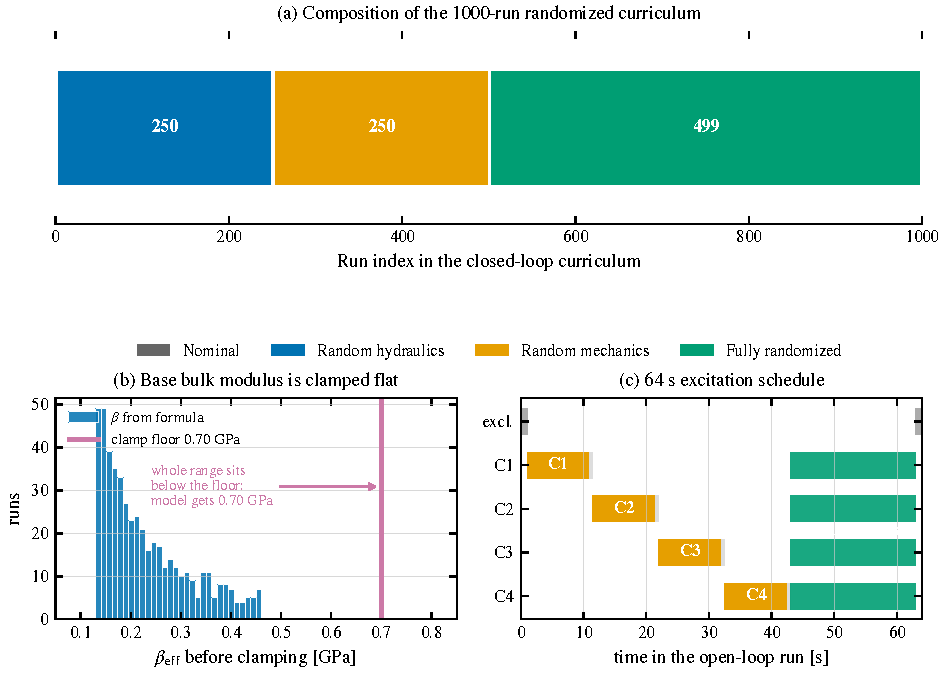
\includegraphics[width=\textwidth]{images/ch4_dataset_design}
  \caption{Design of the two collection campaigns.
  (a)~Composition of the closed-loop curriculum: one nominal run, then $250$
  hydraulics-only, $250$ mechanics-only and $499$ fully randomized draws.
  (b)~Timeline of one open-loop excitation run.}
  \label{fig:data:design}
\end{figure}

\subsection{Hydraulic Parameters}

Table~\ref{tab:data:hydraulic} lists the hydraulic axes. They were
chosen to correspond to the physical mechanisms that make one machine
differ from another in service, in the sense discussed in
Section~\ref{sec:fund:actuation-chain}: air works its way into the
fluid, spools and seals wear, and relief settings drift.



The seal-wear coordinate deserves comment because it is the one place
where a single sampled number is deliberately allowed to move several
model parameters together. A worn cylinder does not become leakier
without also becoming slower, so $w_{\mathrm{seal},i}$ scales the piston
clearance linearly, the valve leakage area with the cube of the same
factor, and the spool time constant from $\unit[8]{ms}$ to about
$\unit[13]{ms}$ at the top of the range. Sampling those three
independently would have produced physically incoherent machines, some
of them very leaky and yet perfectly fast.

\subsection{The Compressibility Axis}
\label{sec:data:compliance}

The entrained-air and dead-volume coordinates randomize the chamber dead
volume, which spans $505$ to $\unit[579]{mL}$ across the batch. This reaches
the pressure dynamics through the continuity equation
\eqref{eq:sys:continuity}, which carries the chamber volume: a larger chamber
is more compliant and slower, a smaller one stiffer and faster. The
compressibility axis therefore enters the batch as capacitance variation.

\subsection{Mechanical Parameters}

The mechanical axes, listed in Table~\ref{tab:data:mechanical}, are
applied to all fourteen rigid bodies of the mechanism: the six links,
the four cylinder barrels, and the four pistons. For each body the mass
is perturbed by up to $\pm 20\,\%$, the centre of mass by up to
$\pm 5\,\%$ of its nominal offset, and the inertia tensor together with
its products of inertia is perturbed consistently with the mass change,
so that the body remains physically realisable rather than acquiring an
inertia that its mass could not produce.



The joint stiffness and damping terms model compliance in the bearings
and linkage rather than in the fluid. They matter here because they set
how much of a pressure transient appears as boom oscillation instead of
clean motion, which is the coupling that a purely kinematic
controller cannot anticipate.

\section{Closed-Loop Data Collection}
\label{sec:data:closed-loop}

The complete closed-loop procedure is summarized in
Algorithm~\ref{alg:data:closed-loop}. Two features stand out before the prose expands on them: the parameter table is
drawn in full before any simulation runs, so the plant family is fixed
and reproducible independently of the collection, and the reference
trajectory is resampled inside every run, so no two runs share a path.

\begin{algorithm}[tb]
  \small
  \DontPrintSemicolon
  \SetKwInOut{Input}{input}\SetKwInOut{Output}{output}
  \Input{run budget $N=1000$; joint limits $\bm{q}_{\min},\bm{q}_{\max}$;
    nominal parameters $\bm{\theta}_0$}
  \Output{dataset $\mathcal{D}=\{(\text{trajectory}_i,\bm{\xi}_i)\}_{i=1}^{N}$}
  \BlankLine
  $\mathbf{L}\leftarrow\textsc{LatinHypercube}(N,12)$
    \tcp*{one design for the whole batch}
  \For{$i\leftarrow 1$ \KwTo $N$}{
    assign $i$ to a curriculum block (nominal / hydraulic / mechanical /
      full)\;
    $\bm{\xi}_i\leftarrow\textsc{DrawParameters}(\mathbf{L}_i,\text{block})$
      \tcp*{$\varepsilon_{\mathrm{air}},\varepsilon_{\mathrm{vol}},c_d,
      w_{\mathrm{seal}},p_{\mathrm{set}}$; masses, CoM, inertia,
      stiffness}
  }
  \For{$i\leftarrow 1$ \KwTo $N$}{
    inject $\bm{\xi}_i$ into the Simscape model\;
    $n_w\leftarrow\textsc{RandInt}(12,20)$;\quad
      $\bm{W}\leftarrow\textsc{LatinHypercube}(n_w,\text{JDOF})$ within
      $[\bm{q}_{\min},\bm{q}_{\max}]$\;
    assign each segment a speed class (slow / medium / fast / variable);
      \textbf{no} dwell\;
    $\bm{q}_{\mathrm{ref}}(t)\leftarrow\textsc{Interpolate}(\bm{W})$ over
      $\unit[22]{s}$\;
    simulate with \texttt{ode23t}; log on the $\unit[0.05]{s}$ grid\;
    store $(\bm{u},\bm{x},\dot{\bm{x}},\Delta\bm{p},\bm{F},\bm{q},
      \dot{\bm{q}},\bm{q}_{\mathrm{ref}},\bm{\xi}_i)$\;
    \lIf{$i \bmod 100 = 0$}{checkpoint $\mathcal{D}$ to disk}
  }
  \caption{Closed-loop curriculum generation.}
  \label{alg:data:closed-loop}
\end{algorithm}

\subsection{The Controller as a Data-Collection Instrument}

Every closed-loop run is driven by the same fixed integral-backstepping
controller, operating on all five joints at a $\unit[0.005]{s}$ rate.
Its gains are never retuned between runs. This is deliberate: the
controller is here as a standardised instrument for putting the arm
through realistic motion, not as a control contribution of this thesis,
and holding it fixed is what makes the resulting behavioural differences
attributable to the plant draw rather than to the controller.

Three details of the controller matter later. The second joint carries
the gravity load of the whole boom, so it is handled by a
proportional-integral law with velocity damping and an explicit gravity
bias rather than by the backstepping law used on the others. A barrier
term keeps the commanded configuration away from the joint limits
imported from the URDF. And the commands are saturated per axis at
$[0.95,\, 0.95,\, 0.80,\, 0.80,\, 0.90]$. That last vector matters: the first four entries are exactly the clip limits stored in the
inverse-dynamics checkpoint in Section~\ref{sec:models:id}. The ID
network inherited its output limits from the instrument that generated
its training labels, which is correct but easy to mistake for a
free design choice.

\section{Open-Loop Excitation Experiments}
\label{sec:data:open-loop}

\subsection{Limitations of the Closed-Loop Batch}

The first forward-dynamics model was trained on the closed-loop material
and scored a one-step $R^2$ near $0.999$. It was also, as
Section~\ref{sec:models:fd-identifiability} documents, almost completely
insensitive to its own valve input: zeroing that input changed the
long-horizon rollout error by a few percent. The model had learned to
continue a trajectory, not to respond to a command.

This is not a training failure and no amount of retraining on the same
material would have fixed it. In closed loop the controller computes the
command from the state, so the command is very nearly a deterministic
function of the state history that the network already
sees~\cite{ljung1999system}. The information needed to separate cause
from correlation is simply not present in the data. Recovering it
requires an experiment in which the command is generated independently
of the state, which means opening the loop.

This is not a coverage problem in disguise.
Figure~\ref{fig:data:regimes} shows that the closed-loop batch is in
fact varied in its control effort: pooled over a run, the valve spends
about a quarter of the time saturated, roughly half in the mid-authority
band, and the rest in low-command creep, so all three control regimes
are represented. The difficulty is visible in the same figure. Plotting
the valve command against the cylinder velocity it produced shows the
two riding together along a band rather than filling the plane: in a
feedback loop a fast motion is when the controller commands a
large valve opening, so command and state move as one. A model can read
the command off the velocity, which is why it never has to learn what
the command \emph{causes}. Diverse control effort and identifiable
control effort are not the same thing, and this batch has the first
without the second.

\begin{figure}[tb]
  \centering
  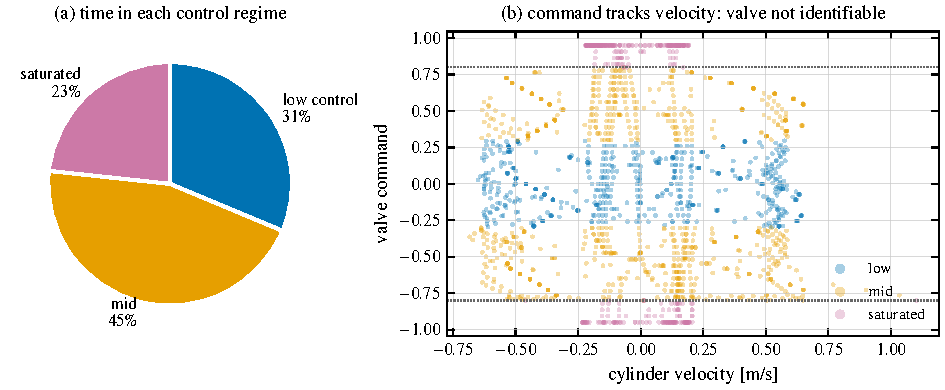
\includegraphics[width=\textwidth]{images/ch4_regimes}
  \caption{The closed-loop batch is diverse in control effort but
  not identifiable. (a)~Fraction of time the valve spends saturated, in the mid
  band and in low-command creep. (b)~The same run in the command--state plane,
  where the correlation that blocks identification is visible.}
  \label{fig:data:regimes}
\end{figure}

\subsection{Design of the Excitation Signal}

The excitation run lasts $\unit[64]{s}$ and follows the fixed schedule
in Figure~\ref{fig:data:design}(c). One second of startup is simulated
and then discarded, because the plant is settling from its initial
condition and those samples describe the initialisation rather than the
dynamics. Four sequential slots follow, each giving one cylinder ten
seconds of excitation followed by a half-second zero-command gap. The
gaps make the boundaries between single-axis segments unambiguous. A
twenty-second phase then drives all four channels at once, and a final
second of zero command closes the run. Commands are limited to
$\pm 0.90$ of full authority.

The most consequential design decision here is one that runs against the
textbook reflex. A persistently exciting input for a linear system is
usually a rapidly switching signal, and the first version of this
excitation was built that way. It was persistently exciting in the
formal sense and still produced poor data, because the cylinders
reversed before they had travelled anywhere: the commanded energy went
into repeatedly accelerating and decelerating the piston near one point
of the stroke instead of moving it through the workspace. The present
signal replaces fast switching with long full-authority plateaus during
the sequential phase and a slow, high-authority component during the
simultaneous phase, so that each cylinder traverses a
substantial part of its stroke while its valve is open. The simultaneous
phase additionally superimposes one slow near-square cycle across the
full twenty seconds with a distinct medium-frequency component on each
channel, and short raised-cosine ramps at entry and exit keep the
transitions differentiable.

The lesson generalises, and it is one this thesis would offer to anyone
identifying a hydraulic actuator: persistent excitation is a condition
on the input signal, but the quantity that decides whether a
\emph{cylinder} is identifiable is how much of the stroke the input covers. The two are not the same, and optimising the first
while ignoring the second produces data that passes the classical test
and still cannot support a model.

\subsection{Plant Draws and Acceptance}

The same excitation is applied to four plant draws taken from the same
parameter space as the closed-loop campaign: nominal, randomized
hydraulics, randomized mechanics, and fully randomized. Holding the
input fixed and varying only the plant is what makes the four runs
directly comparable, since any difference in the response is attributable
to the parameters.

Each run is checked for stroke coverage before it is accepted. The
collector requires at least $10\,\%$ of the available stroke on
cylinders 1--3 and $8\,\%$ on cylinder 4, warns below a target of
$30\,\%$, and records the achieved coverage per channel in the run
summary. The runs retained here cover between $12\,\%$ and $33\,\%$ of
the stroke depending on the cylinder, which is above the acceptance
floor but below the target. Cylinder 4 is the weakest, and improving its
coverage is the clearest available next step for this campaign.

One earlier excitation export was rejected outright rather than repaired.
Half of its runs turned out to contain duplicated state trajectories, so
the nominally distinct plant draws were not distinct in the data, and
the valve was again not causally identifiable. That export and its
reports are not part of the maintained workflow. It is mentioned here
because it is the reason the acceptance checks in
Section~\ref{sec:data:diagnostics} exist in their present form: they were
written to make that particular failure impossible to miss a second
time.

\section{Combining Closed-Loop and Open-Loop Datasets}
\label{sec:data:combining}

The two campaigns are complementary, and each learned model of
Chapter~\ref{chap:models} draws on them in a different proportion.

The inverse-dynamics model is trained entirely on closed-loop material,
because its target is the command a competent controller issued in a given
state. The forward-dynamics model begins there and is then retrained on the
strict open-loop export, with the closed-loop data retained as a replay term at
weight $0.25$. Ablation showed that dropping the replay term costs state
coverage and extension accuracy, because four excitation runs cannot span the
poses a thousand operating runs visit.

Figure~\ref{fig:data:coverage} shows why. The closed-loop distribution fills
the reachable range smoothly; the open-loop distribution concentrates into
narrow plateaus. The open-loop bands are where the valve is identifiable, the
closed-loop mass is where the model must be accurate at deployment, and neither
campaign covers both. The forward model is therefore trained on their union.

\begin{figure}[tb]
  \centering
  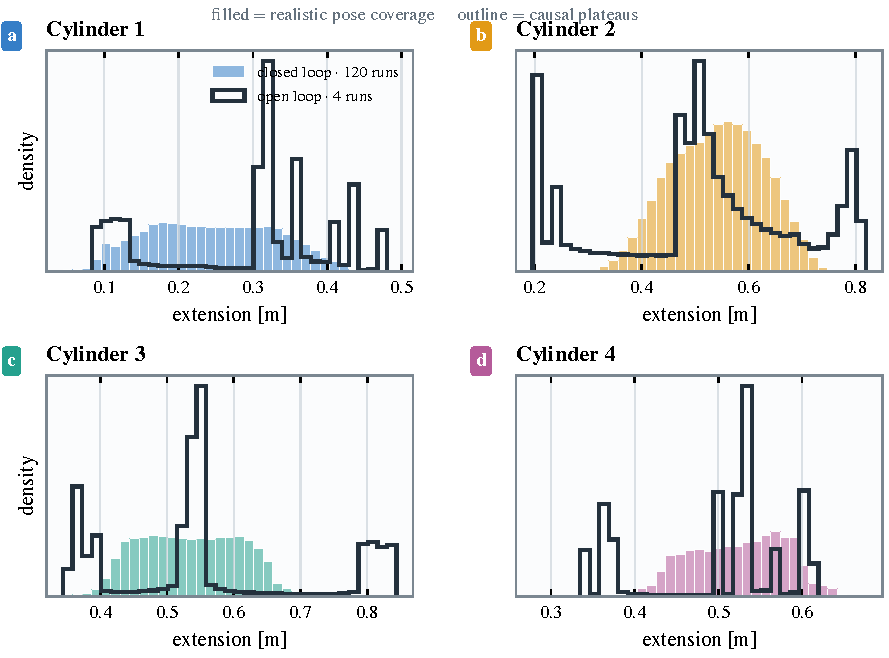
\includegraphics[width=\textwidth]{images/ch4_coverage}
  \caption{Extension coverage of the two campaigns, per cylinder
  and pooled over runs (closed-loop filled, open-loop outline). The closed-loop
  data fills the reachable range smoothly; the open-loop data concentrates into
  the plateaus where the valve is identifiable.}
  \label{fig:data:coverage}
\end{figure}

The reduced-order model consumes the closed-loop material in a joined
form. The inverse and forward exports are aligned on exact run
identifiers, time indices, and sample times, and the join is accepted
only when the sixteen-dimensional cylinder state agrees between them
sample for sample. The resulting command-conditioned dataset contains
$452\,400$ transitions at $\unit[0.05]{s}$ drawn from $1\,040$ aligned
runs. The logged valve command is carried through this join, but only as
a supervision target for the model's internal valve head. It is never a
runtime input, which is the property that lets the ROM be driven by
desired cylinder motion alone (Section~\ref{sec:models:rom}).

The thousand-run randomized curriculum described in
Section~\ref{sec:data:closed-loop} occupies a different position in the
argument, and I want to be exact about it because it is easy to
overstate. The inverse, forward, and reduced-order models reported in
Chapter~\ref{chap:models} were trained on the earlier aligned export,
which is a nominal-plant collection. The randomized curriculum was
collected under the earlier plan, in which randomized Simscape runs
would supply both the robust actuator variants and the privileged
factor vectors for latent adaptation. Neither role survives: the
adaptation evidence chain of this thesis is built entirely on the
IsaacLab collection of Section~\ref{sec:data:isaaclab}, for the reason
given there, and no result in this thesis is trained on or evaluated
against the randomized Simscape curriculum. It is reported as
provenance and as a negative methodological record, not as a substrate
whose consequences appear later.

\section{Closed-Loop Calibration Data for the Command ROM}
\label{sec:data:rom-calibration}

The reduced-order model is the one actuator model that does not stop at the
Simscape boundary. It is accurate about hydraulics, but the plant it drives at
runtime is a PhysX articulation with its own contact behaviour and compliance,
and the systematic offset between the extension the ROM commits to and the one
PhysX realizes is invisible to any amount of further Simscape training.

The calibration set is therefore collected from the deployment loop itself. A
previous ROM checkpoint is rolled out through the parked workflow of
Section~\ref{sec:sys:parked} on its five reference shapes, logged on the ROM's
own $\unit[0.05]{s}$ grid, giving $4\,084$ transitions. Each record stores the
six-step ROM history as the runtime assembles it, together with the measured
PhysX transition. The targets are what the plant did, not what Simscape said it
would do.

Two properties make the set safe to use. Only the bounded command-gated
correction head is trainable against it, with every other parameter frozen and
the correction capped at $\unit[3]{mm}$, so the identified physics is preserved
and only a deployment offset is added. And fine-tuning runs against a mixture,
replaying the original dataset at weight $0.25$, because five parked shapes
cannot span the poses a thousand Simscape runs visit. The correction is
command-gated and therefore exactly zero at zero command, so the stationary
hold contract survives unchanged.

One limitation is carried forward. The calibration data comes from the
\emph{parked} diagnostic workflow rather than the moving-verge task, so it
fits the actuator to PhysX under free-space tracking and not under
cutter--ground contact. The calibration is therefore weakest in the regime the
verge task spends most of its time in, and the bounded correction head keeps
that gap contained rather than closing it. This calibration is also what
qualifies the ROM as the deployment actuator, with the consequences for the
three-way comparison set out in Section~\ref{sec:sys:rom-is-plant}.

\section{The IsaacLab Adaptation Collection}
\label{sec:data:isaaclab}

\subsection{Provenance of the Adaptation Data}

The models that carry the adaptation argument
(the system-dynamics surrogate, the privileged factor encoder, and the
AAM) describe the plant that the adaptive controller is closed around. That
plant is not the Simscape model. It is the command ROM plus PhysX, the
same four-dimensional cylinder command port used at deployment. A
surrogate identified on Simscape data would be a model of a model, and
the latent it defines would describe variation the deployment plant does
not necessarily exhibit. The adaptation dataset is therefore collected
\emph{in} the deployment plant, and the frozen ROM, ID and FD
checkpoints enter this chain only as fixed components, never as things
to be retrained.

\subsection{The Physical Factor Vector}
\label{sec:data:factors}

The randomized quantity is a six-dimensional physical factor vector
%
\begin{equation}
  \label{eq:data:factorvec}
  \factorvec = \bigl[
    e_{\mathrm{flow}},\;
    e_{\mathrm{compliance}},\;
    e_{\mathrm{seal}},\;
    e_{\mathrm{pressure}},\;
    e_{\mathrm{mass}},\;
    e_{\mathrm{COM}_z}
  \bigr],
\end{equation}
%
with the ranges of Table~\ref{tab:data:factors}. Four coordinates are
hydraulic and two mechanical, which is what makes the hydraulic-only,
mechanical-only, and combined domains of
Section~\ref{sec:data:domains} separable. Each candidate was admitted
only after a one-factor sensitivity screen confirmed that moving it
alone produces a measurable change in cylinder extension, velocity,
pressure, or end-effector motion. Parameters whose effect could not be
measured, or which could not be varied safely, were rejected rather than
carried as decoration.



One omission is deliberate. Actuation delay is not a
randomized coordinate. Delay in this system is an \emph{emergent}
property of flow, compliance, and load rather than a free parameter, so
it is measured as a response property of each run
(Chapter~\ref{chap:evaluation}) instead of being supplied to any model
as a known factor. Handing an estimator a factor that the real machine
would never publish is the same mistake as handing it the true latent.

\subsection{Domains and Factor Design}
\label{sec:data:domains}

Runs are organized into five domains
(nominal, hydraulic-only, mechanical-only, combined-training, and an
\emph{unseen} combined-test domain), and one factor vector is fixed for a complete run, so that no
run mixes plants. Factor configurations are drawn with deterministic
scrambled Sobol sequences~\cite{sobol1967distribution} rather than
independent uniform sampling, with explicit boundary anchors so that the
corners of the space are represented and not merely approached, and with
fixed per-domain seeds so the design is reproducible independently of
the data it produced. Combined draws that compound into an excessive
response gain are rejected at draw time rather than being collected and
discarded later.

The resulting design is auditable: $98.3\,\%$ of the factor keys are
unique, the active-factor matrix is full rank, every factor quartile is
populated, and the factor keys of the training, validation, and test
splits are disjoint. That last property is the one that matters most for
the claims of Chapter~\ref{chap:evaluation}: a test run does not merely
come from a different episode, it comes from a plant the models have
never seen.

\subsection{Collection Procedure}

Every run is collected through the same interface the policy uses. The
DLS controller closes the loop on measured cylinder state and issues its
command through the four-dimensional action port into the command ROM
and PhysX. No joint-target bypass is used, and no PPO policy is used to
collect identification data, because a policy trained on the same plant
would reintroduce the closed-loop correlation that
Section~\ref{sec:data:open-loop} spent a campaign removing.

Independent excitation is supplied by dedicated four-channel PRBS
windows applied through that same action port, with a small amplitude
and a hold of ten control steps, so that the excitation is causally
independent of the state without ever leaving the safe envelope. Probe
actions are logged separately from controller output, so any analysis
can distinguish the two. Each run follows a fixed eleven-segment structure
(settle, three postures, three PRBS windows, DLS task motion,
reach-and-return, and stow), giving $11\,304$ control steps
and $\unit[188.4]{s}$ of simulated time per run. Three postures plus
line, coupled-sine, and reach-and-return motion were verified in a pilot
to give full rank over all four action channels under varied geometry
and load.

\subsection{The Frozen Dataset}

The final collection contains $118$ complete runs: $2$ nominal, $40$
hydraulic-only, $12$ mechanical-only, $48$ combined-training, and $16$
unseen combined-test. Collection ran in four vectorized IsaacLab
environments with per-environment factors and logging. Slots that
tripped a safety or validity check were discarded and retried
individually rather than being silently kept. All $118$ runs passed the
final collection gate, which checks finite physics, exact model-grid
alignment, command rank, factor-response authority, state coverage, and
saturation limits.

The dataset is then \emph{frozen}: the raw runs are checksummed and the
run-level split is fixed at $82$ training, $20$ validation, and $16$
reserved combined-test runs, with zero factor-key leakage between them.
The reserved sixteen are not touched again:
not for history-length selection, not for model selection, and not for
hyperparameter choices, so that the final adaptation claim is measured on material no decision
in this thesis was conditioned on.

\subsection{Learning Timebase and Hydraulic State}

The learning timebase is the actuator model grid, not the control clock.
Samples are exact $\unit[50]{ms}$ ROM transitions taken at control
indices $0, 3, 6, \dots$: state row $t$ and command row $t$ predict
state row $t+3$. Nothing is interpolated. This is the same alignment
rule as Section~\ref{sec:sys:timing}, and it is enforced rather than
assumed, because a model trained across a mismatched interval is wrong by a fixed factor in the quantity it exists to supply.

The hydraulic state used by the system-dynamics models is
%
\begin{equation}
  \label{eq:data:sdstate}
  \bm{s}_t = \bigl[\bm{x}_t^{1:4},\; \dot{\bm{x}}_t^{1:4},\;
  \Delta\bm{p}_t^{1:4}\bigr] \in \mathbb{R}^{12},
\end{equation}
%
with joint position and velocity carried as \emph{context} only, and the
prediction target the next $\unit[50]{ms}$ state delta. Differential
pressure occupies an awkward position in this design: it is
recorded, and it is a prediction target and a diagnostic, but it is
withheld from the final deployment-mirror input. A real machine does not
publish chamber pressure on this interface, so a model allowed to read
it would be validated under an assumption deployment cannot honour.
Withholding it is what makes a causal history \emph{belief} necessary
rather than optional, and that necessity is the whole reason the AAM has
work to do.

\section{Feature and Target Construction}
\label{sec:data:features}

\subsection{The Actuator Models}

The three learned actuator models take cylinder-space features, in the
ordering and notation fixed in Section~\ref{sec:models:overview}. Their
input contracts differ because their questions differ. The inverse model
receives the measured cylinder state, the logged rod forces, the desired
increments, and the previously applied command, twenty-eight numbers in
all. The forward model receives the applied valve command and the
measured state, twenty numbers. The reduced-order model receives a
six-sample history of state, previously predicted valve, and desired
command, twenty-four numbers per step.

Three conventions apply throughout, and they are the same ones the models
enforce at inference time.

\paragraph{Increment Targets}
Every dynamic target is a within-run one-step increment,
$\Delta \bm{x}_k = \bm{x}_{k+1} - \bm{x}_k$, never an absolute state.
This removes the large static component of the signals and, more
importantly, makes the trivial persistence solution an explicit baseline
that a model can be measured against rather than a hiding place it can
settle into.

\paragraph{Causal Alignment}
Features at step $k$ contain only quantities available at step $k$. The
extraction stage verifies this by recomputing every logged target from
the within-run difference of the states and requiring exact agreement,
a check reported in Section~\ref{sec:data:diagnostics}.

\paragraph{Time-Base Conversion}
The open-loop campaign is logged at $\unit[0.01]{s}$ but the models run
at $\unit[0.05]{s}$, so five consecutive raw samples are combined into a
single transition. The valve input attributed to that transition is the
command held at the start of the window, which is the causally correct
choice. The mean command over the window is also recorded, but only for
analysis. Cylinder extension velocity is not logged directly in the
closed-loop archive and is obtained by differentiating extension on the
output grid, which is consistent with the trapezoidal identity that the
strict data satisfies to $R^2 = 0.994$--$0.9997$
(Equation~\ref{eq:models:trapezoid}).

\subsection{Observable History of the Adaptation Models}
\label{sec:data:history-features}

The adaptation models draw their features from the frozen IsaacLab
collection, and here the interesting question is not what goes in but
what is kept out. A history window carries only quantities a deployed
machine could produce: the applied action, cylinder extension and
velocity, and joint position and velocity. Six classes of signal are
excluded by construction, and the exclusion is enforced by an explicit
input mask rather than by convention:

\begin{itemize}
  \item the physical factors $\factorvec$ and the true latent $\bm{z}$,
    because recovering them is the estimator's job;
  \item any future observation, because the estimator is causal;
  \item the hidden internal state of the command ROM, because the
    deployment interface does not expose it;
  \item the differential pressure $\Delta\bm{p}$, for the reason given
    in Section~\ref{sec:data:isaaclab};
  \item the desired task reference, so that the latent describes the
    plant rather than the trajectory being asked of it.
\end{itemize}

Windows are contained within a single run and never cross a run
boundary, and each window carries the stopped-gradient target
$\bm{z} = \mu(\factorvec)$ of its own run together with the run
identifier, domain, split, and valid history bounds. Applied to the
$118$ frozen runs this yields $444\,624$ causal history ticks. What is
built from them, how the history length is chosen, and how the result is
validated downstream belong to Chapter~\ref{chap:models}.

\section{Preprocessing and Data Splits}
\label{sec:data:preprocessing}

Splitting is done at the level of complete runs, never of individual
samples. A random sample-level split would place transitions from the
same trajectory on both sides of the boundary and report a validation
score that mostly measures interpolation within a run. For the
command-conditioned dataset the $1\,040$ runs are divided into $936$
training, $52$ validation, and $52$ test runs, giving $407\,160$,
$22\,620$, and $22\,620$ transitions respectively, with no run
identifier appearing in more than one split. The IsaacLab adaptation
collection is split by run \emph{and} by factor configuration
($82$/$20$/$16$, Section~\ref{sec:data:isaaclab}), which is the stronger
condition: separating runs alone would still let two runs of the same
plant fall on opposite sides of the boundary and turn a claim about
unseen plants into a claim about unseen episodes.

The strict open-loop export needs a different treatment because it
contains only four runs, and holding one out would remove an entire
plant draw from training. Instead each run is divided into twenty
temporal blocks, every fifth block is assigned to validation, and a
five-sample guard interval is discarded at each block boundary so that
no $\unit[0.05]{s}$ transition window spans the split. A simple
last-twenty-percent split was tried first and rejected: it changed the
spread of the targets between training and validation by a factor of
$1.3$ to $2.3$, because the final fifth of the run is the simultaneous
excitation phase and is dynamically unlike everything before it. That
split would have measured extrapolation to a different regime and called
it generalisation.

Normalization statistics are computed on the training split only and
stored inside each checkpoint, so that a model always normalizes with the
statistics it was fitted with. Mixing statistics between checkpoints
silently invalidates any comparison, and the loader enforces the stored
contract rather than recomputing it.

Finally, samples are carried with an explicit validity flag rather than
being silently dropped. In the strict export $93.7\,\%$ of samples are
marked valid. The remainder are the excluded startup and shutdown
seconds and the zero-command gaps. Keeping them in the archive with a
flag, instead of deleting them, means the time base stays contiguous and
the within-run difference checks remain meaningful.

\section{Dataset Diagnostics}
\label{sec:data:diagnostics}

No dataset in this thesis is used before it passes an explicit audit,
for the reason given at the end of
Section~\ref{sec:data:open-loop}. The audit of the strict open-loop
export is reproduced in Table~\ref{tab:data:audit}.



The two rank figures are the ones that speak directly to requirement R2.
The instantaneous command matrix has rank four, so no channel is a
linear combination of the others, and the lagged regressor matrix built
from the command history has rank eighty, so the excitation is
persistently exciting to the order the models need. The condition number
of that lagged matrix is about $4.6\times10^{3}$, which is finite and
workable rather than comfortable. It is a consequence of using long
plateaus, and it is the price paid for the stroke coverage those
plateaus buy.

The exactness of the three increment checks deserves a word, since a
maximum error of exactly zero invites suspicion. It is expected here:
the targets are computed from the logged states by the same within-run
difference that the check recomputes, so the check verifies that the
extraction stage did what it claims, not that the simulation is
accurate. It catches misalignment, off-by-one indexing, and rows that
have been reordered or concatenated across run boundaries, which are the failure modes that occur. Physical fidelity is a separate
question, addressed by the validation study in
Section~\ref{sec:sys:simscape-validation}.

Three limitations of the Simscape material are carried forward honestly.
Two limitations are carried forward. Stroke
coverage reaches only $12\,\%$ on the head-pivot cylinder, which is also the
cylinder the strict forward model predicts least well. The rod-force channel
fails a piston-area consistency check on this export, so it carries zero
supervised weight in the reduced-order model and no result rests on it.

The IsaacLab collection is audited against different failure modes. Design
adequacy is checked before use (unique factor keys, full active-factor rank,
disjoint keys across splits), physical validity per run (finite physics, exact
model-grid alignment, full command rank, bounded saturation), and leakage
structurally, with privileged channels removed by an explicit input mask rather
than by trusting the feature list. Its limitation is scale: $118$ runs over six
factors is a sparse design, which is why the adaptation claims of
Chapter~\ref{chap:evaluation} are reported with paired bootstrap intervals and
per-run detail rather than pooled point estimates.

With the data described and audited, the next chapter turns to what was
learned from it: the inverse and forward models that form the
\ppoIDFD{} actuator path, the command-conditioned reduced-order model
that replaces them in \ppoROM, and the system-dynamics, encoder, and
adaptation models built on the IsaacLab collection.
